\documentclass{beamer}

\usepackage{idrislang}
\usepackage{amsmath}
\usepackage{listings}
\usepackage{bussproofs}
\usepackage{tikz}
\usepackage{tikz-cd}

\usetheme{Szeged}
\usecolortheme{dolphin}

\title{An Introduction to Functional Programming}
\author{Thomas E. Hansen}
\institute{University of St Andrews}
\date{\today}

\begin{document}
\begin{frame}[plain]
  \titlepage
\end{frame}

\begin{frame}
  \frametitle{Overview}
  \tableofcontents
\end{frame}

\section{Introduction}
  \subsection{About}
  \begin{frame}
    \frametitle{About...}
    \begin{itemize}
      \item ... this talk
            \begin{itemize}
              \item This is a talk about functional programming
              \item It assumes no pre-existing knowledge
              \item I've tried to aim it at people with knowledge of imperative
                    languages
            \end{itemize}
      \item ... me!
            \begin{itemize}
              \item I'm Thomas/Tom
              \item I work with Edwin Brady
              \item I'm interested in formal methods, low-level programming,
                    making software provably robust/correct, etc.
            \end{itemize}
    \end{itemize}
  \end{frame}

  \subsection{What do we mean by `functional'?}
  \begin{frame}
    \frametitle{What do we mean by `functional'?}
    \begin{itemize}
      \item As opposed to what? Non-functional?...
      \item Ask 100 functional programmers, get at least 100 different answers
      \item Functions should be \textit{first-class}
        \begin{itemize}
          \item Can be assigned to variables, passed to other functions, stored
                in data structures, etc., just like other first-class things,
                e.g. numbers
          \item Python and JavaScript allow this, but would not typically be
                called `functional' languages
        \end{itemize}
      \item The language should encourage some ``functional programming style''
        \begin{itemize}
          \item More on this shortly
        \end{itemize}
    \end{itemize}
  \end{frame}
%  \begin{frame}
%    \frametitle{Imperative vs Functional}
%    \begin{itemize}
%      \item Imperative
%        \begin{itemize}
%          \item Define a lot of details on \textit{how} to do things
%          \item What to refer to memory as (e.g. variables and classes)
%          \item How to operate on the memory, how to update it, etc
%        \end{itemize}
%      \item Functional
%        \begin{itemize}
%          \item Define the details of \textit{what} to do
%          \item ``Given this input, the output looks like [...]''
%          \item The idea being that humans are better at reasoning about this
%          \item Leave the memory management and similar details to the
%programming
%                language implementation and runtime
%        \end{itemize}
%    \end{itemize}
%  \end{frame}

  \subsection{What FP doesn't have to be}
  \begin{frame}[fragile]
    \frametitle{It doesn't have to be like this}
    \begin{columns}[c]
      \tiny
      \column{0.5\textwidth}
        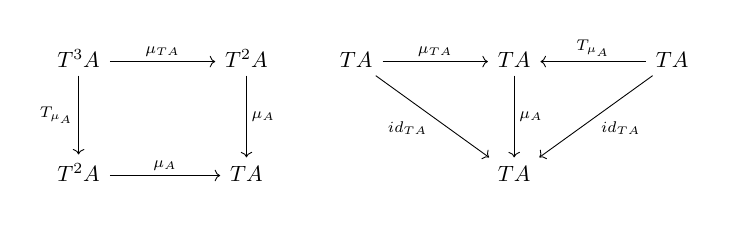
\begin{tikzpicture}
          \node[scale=0.8]{
          % drawn using https://tikzcd.yichuanshen.de/
          \begin{tikzcd}
            T^3A \arrow[dd, "T_{\mu_{A}}"'] \arrow[rr, "\mu_{TA}"] &  & T^2A \arrow[dd, "\mu_A"] & TA \arrow[rr, "\mu_{TA}"] \arrow[rrdd, "id_{TA}"'] &  & T²A \arrow[dd, "\mu_A"] &  & TA \arrow[lldd, "id_{TA}"] \arrow[ll, "T_{\mu_{A}}"'] \\
                                                                   &  &                          &                                                    &  &                         &  &                                                       \\
                                                                   T^2A \arrow[rr, "\mu_A"]                               &  & TA                       &                                                    &  & TA                      &  &
          \end{tikzcd}
          };
        \end{tikzpicture}

        \vspace*{7mm}

        {\small ``A monad is just a monoid in the category of endofunctors,
        what's the problem?''}

        \begin{prooftree}
          \AxiomC{$\Delta_0 \vdash \rho\ f \in (\pi x : S) \rightarrow T$}
          \AxiomC{$\Delta_1 \vdash \rho \pi\ S \ni s$}
          \BinaryInfC{$\Delta_0 + \Delta_1 \vdash \rho f s \in T[s: S/x]$}
        \end{prooftree}

      \column{0.5\textwidth}
        \centering
        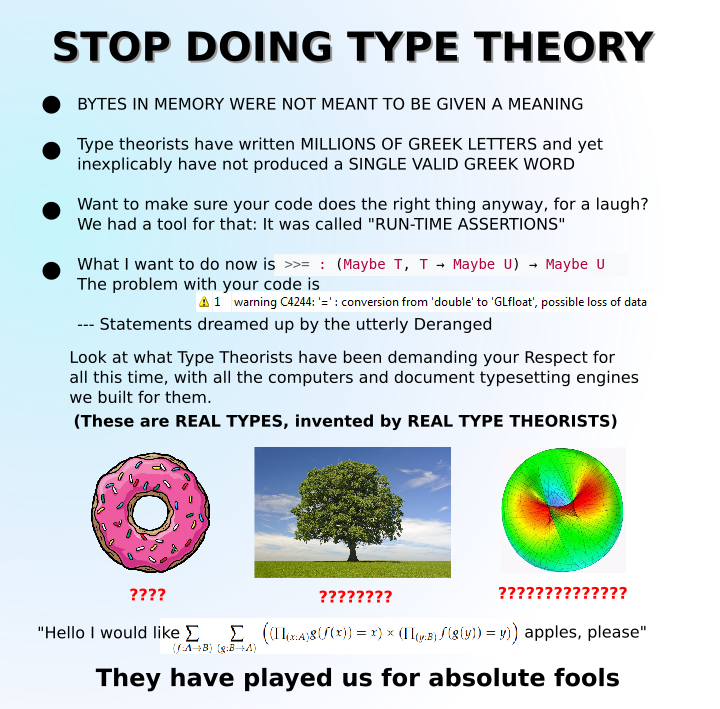
\includegraphics[width=\textwidth]{stop-doing-type-theory.png}
        \tiny\color{gray}\url{https://twitter.com/jcreed/status/1367899760301137930}
    \end{columns}
  \end{frame}


\section{Imperative vs Functional}
  \subsection{Types}
  \begin{frame}
    \frametitle{Types}

    \begin{itemize}
      \item Types define sets of things
      \begin{itemize}
        \item `\texttt{int}' or `\texttt{Int}' denotes the set of integers
        between $-(2^{31})$ and $2^{31} - 1$ (typically)
        \item `\texttt{String}' denotes the infinite set of all possible strings
      \end{itemize}
      \item In Java, we have \texttt{int}, \texttt{bool}, \texttt{String}, etc.
      \item In functional programming, we have these but we also have more
      complicated types:
      \begin{itemize}
        \item `\texttt{Int -> Int}' --- the set of functions which take an
        \texttt{Int} and return an \texttt{Int}
        \item `\texttt{Type -> Type}' --- the set of functions which convert one
        type to another (types are also first-class!)
      \end{itemize}
      \item We write ``\texttt{name : T}'' to say ``\texttt{name} has type
      \texttt{T}''
    \end{itemize}

  \end{frame}

  \begin{frame}
    \frametitle{Types are useful!}

    \begin{itemize}
      \item Languages like Java, C++, Haskell, Idris, etc. are ``statically''
      typed
      \begin{itemize}
        \item The compiler complains if we try to pass a `\texttt{String}' as an
        argument to a function that expects an `\texttt{Int}'
        \item Java and C++ automatically cast some numeric types
      \end{itemize}
      \item Languages like Python, Perl, PHP are ``dynamically'' typed
      \begin{itemize}
        \item Different things can be passed to functions regardless of their
        type and errors arise at runtime rather than compile-time
      \end{itemize}
      \item In strongly typed languages, types help us use the functions,
      data-structures, and variables we define correctly
      \begin{itemize}
        \item Like fitting the right shapes in the right holes
      \end{itemize}
    \end{itemize}

  \end{frame}

  \subsection{Functions}
  \begin{frame}[fragile]
    \frametitle{Imperative programming}

    \begin{itemize}
      \item Calculating the power of a number in Java:
            \vspace*{-1mm}
      {\footnotesize
       \begin{lstlisting}[language=java]
public int power(int a, int p) {
  int pow = 1;
  for (int i = 0; i < p; i++) {
    pow = pow * a;
  }
  return pow;
}
      \end{lstlisting}}
      \vspace*{-2mm}
      \item ``A \texttt{public} function, which returns an \texttt{int}, with name
            `\texttt{power}', taking an \texttt{int} referred to as `\texttt{a}'
            and an \texttt{int} referred to as `\texttt{p}' as arguments''
      \item The body defines a lot of \textit{how}:
        \begin{itemize}
          \item Allocate an \texttt{int}-sized bit of memory referred to as
                `\texttt{sum}', store the initial value 1 in it, how to update
                it...
        \end{itemize}
    \end{itemize}

  \end{frame}

  \begin{frame}[fragile]
    \frametitle{Functional programming}

    \begin{itemize}
      \item In Idris:
            \vspace*{-5mm}
      {\footnotesize
        \begin{idrislisting}
export
power : (a : Integer) -> (p : Integer) -> Integer
power a 0 = 1
power a p = a * power a (p - 1)
      \end{idrislisting}}
      \vspace*{-1mm}
      \item The `\texttt{export}' keyword allows for external access
      \item The function `\texttt{power}' has type\\
            `\texttt{Integer -> Integer -> Integer}'
      \item The `\texttt{->}' separates arguments
      \item We can use `\texttt{(a : Integer)}' to give an argument a name
      \item The type after the final `\texttt{->}' is the function's return type
    \end{itemize}

  \end{frame}

  \begin{frame}[fragile]
    \frametitle{Functional programming (cont.)}

    \begin{itemize}
      \item In Idris:
      \vspace*{-5mm}
      {\footnotesize
        \begin{idrislisting}
export
power : (a : Integer) -> (p : Integer) -> Integer
power a 0 = 1
power a p = a * power a (p - 1)
      \end{idrislisting}}
      \vspace*{-1mm}
      \item The function body here uses \textit{pattern-matching}
        \begin{itemize}
          \item Extremely useful!
          \item Allows you to specify function return values in terms of the
                `shape' of the input
        \end{itemize}
      \item If `\texttt{p}' is 0, then the answer is always 1
      \item Otherwise, the answer is $a * a^{p-1}$
        \begin{itemize}
          \item In most FP languages, functions do not take parentheses around
                their arguments (e.g. `\texttt{power 2 2}' would return 4)
        \end{itemize}
    \end{itemize}

  \end{frame}

  \subsection{Data structures}
  \begin{frame}
    \frametitle{Data declarations}

    \begin{itemize}
      \item In Java, we would likely create a class (or an enum)
      \item In Idris, use the `\texttt{data}' or `\texttt{record}' keywords
        \begin{itemize}
          \item \texttt{record} is a data structure with implicit accessors
        \end{itemize}
      \item {\ttfamily
             \underline{data} MyData : Type \underline{where}\\
             \hspace*{1em} NoData : MyData\\
             \hspace*{1em} IntData : (data : Int) -> MyData}
        \begin{itemize}
          \item Declares a new datatype `\texttt{MyData}'
          \item With a constructor `\texttt{NoData}' that takes no arguments
          \item And a constructor `\texttt{IntData}' that takes an argument
                `\texttt{data}' of type \texttt{Int}
        \end{itemize}
      \item There is shorthand for this (with less control)
        \begin{itemize}
          \item {\ttfamily \underline{data} MyData = NoData | IntData Int}
        \end{itemize}
    \end{itemize}
  \end{frame}

  \begin{frame}[fragile]
    \frametitle{Binary trees}

    \begin{columns}
      \column{0.55\textwidth}
      Java:
      {\scriptsize
      \begin{lstlisting}[language=java]
public class Tree<T> {
  public static class Node<T> {
    private T content;
    private Node<T> left;
    private Node<T> right;

    public Node(T elem) {
      this.elem = elem;
      this.right = null;
      this.left = null;
    }
  }
  private Node<T> root;
  ...
}
      \end{lstlisting}
      }

      \column{0.6\textwidth}
      Idris:
      %\vspace*{-6mm}

      \begin{idrislisting}[basicstyle=\ttfamily\scriptsize]
data Tree : (t : Type) -> Type where
  Empty : Tree t
  Node  : (elem : t) ->
          (left : BTree t) ->
          (right : BTree t) ->
          Tree t
      \end{idrislisting}

      \vspace*{1mm}

      {\footnotesize Or, in shorthand form:}

      \vspace*{-2mm}

      \begin{idrislisting}[basicstyle=\ttfamily\scriptsize]
data Tree t
  = Empty
  | Node t (Tree t) (Tree t)
      \end{idrislisting}
    \end{columns}

\end{frame}


\section{Neat and convenient things}
  \subsection{Pattern-matching}

  \subsection{Higher order functions}


\end{document}
